\section{Wpływ algorytmu}
\label{sec:wyniki-wplyw-algorytmu}

Problem badawczy tej pracy obejmuje również wybór samego algorytmu
uczenia przez wzmacnianie, dlatego oprócz wpływu reprezentacji stanu
i funkcji nagrody analizuję również główny efekt algorytmu. Porównałem
REINFORCE z DQN przy zachowaniu tej samej reprezentacji stanu, funkcji
nagrody oraz seedu treningowego. Różnicę zdefiniowałem jako

\begin{equation}
    \Delta EV_{\mathrm{alg}}
    =
    EV_{\mathrm{REINFORCE}}
    -
    EV_{\mathrm{DQN}}.
\end{equation}

Ze wzoru wynika, że wartość dodatnia oznacza przewagę REINFORCE, a ujemna
przewagę DQN. Wyniki wszystkich czterech porównań, z 95-procentowym
przedziałem ufności wyznaczonym z rozkładu $t$-Studenta dla pięciu
sparowanych seedów (podrozdział~\ref{sec:porownania-sparowane}),
przedstawiam w tabeli~\ref{tab:algorithm-effect}.

\begin{table}[htbp]
    \centering
    \caption{Wpływ algorytmu na końcowe EV}
    \label{tab:algorithm-effect}
    \begin{tabular}{llrr}
        \toprule
        Reprezentacja & Nagroda & $\Delta EV_{\mathrm{alg}}$ & 95\% CI \\
        \midrule
        RAW & zysk netto
            & 0{,}2665 & [0{,}2424,\ 0{,}2906] \\
        RAW & skalowana
            & 0{,}1878 & [0{,}1394,\ 0{,}2361] \\
        \midrule
        FEATURES & zysk netto
            & 0{,}0254 & [0{,}0159,\ 0{,}0349] \\
        FEATURES & skalowana
            & 0{,}0954 & [0{,}0046,\ 0{,}1862] \\
        \bottomrule
    \end{tabular}
\end{table}

We wszystkich czterech przypadkach przedział ufności leży całkowicie po
dodatniej stronie zera, co oznacza statystycznie istotną przewagę
REINFORCE nad DQN w podstawowym budżecie 50\,000 epizodów, niezależnie
od zastosowanej reprezentacji stanu i funkcji nagrody. Przewaga ta jest
jednak wyraźnie mniejsza dla reprezentacji FEATURES (0,0254 i 0,0954)
niż dla RAW (0,2665 i 0,1878), co jest zgodne z wynikiem
podrozdziału~\ref{sec:wyniki-reprezentacja-stanu}: reprezentacja
FEATURES poprawiała wyniki DQN znacznie bardziej konsekwentnie niż
wyniki REINFORCE, więc różnica między algorytmami zmniejsza się właśnie
tam, gdzie DQN korzysta z dodatkowych cech domenowych.

Te same porównania przedstawiam także na rysunku~\ref{fig:algorithm-effect}.

\begin{figure}[htbp]
    \centering
    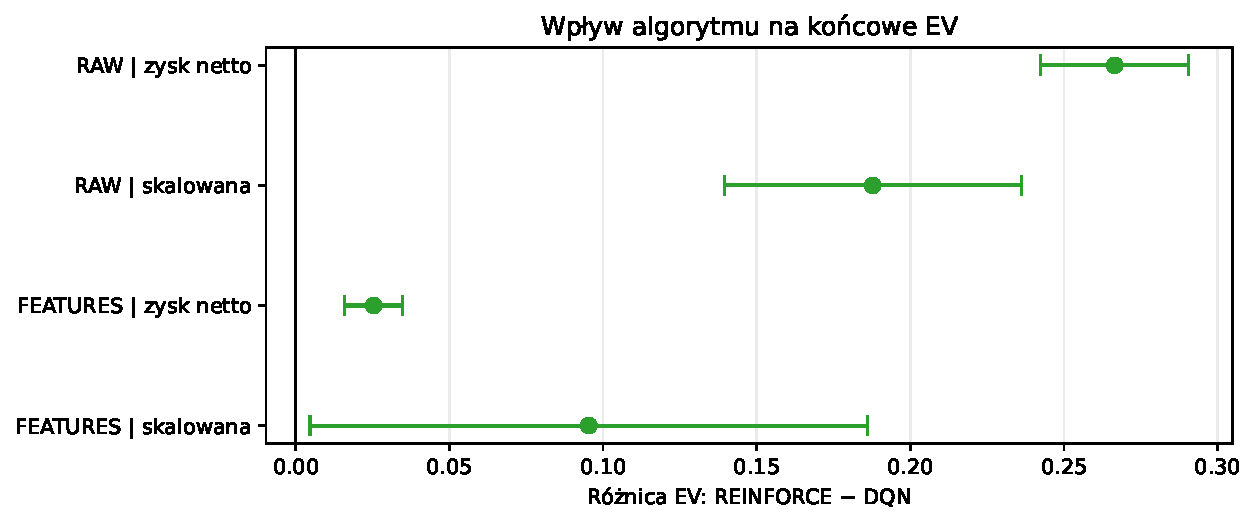
\includegraphics[
        width=0.9\textwidth
    ]{../experiments/results/final_analysis/24_algorithm_effect.pdf}
    \caption{Wpływ algorytmu na końcowe EV}
    \label{fig:algorithm-effect}
\end{figure}

Statystycznie istotna przewaga REINFORCE nie oznacza jednak, że jest to
metoda lepsza pod każdym względem. Jak opisuję w
podrozdziale~\ref{sec:wyniki-zachowanie-polityk}, wyższe średnie EV
REINFORCE było w wielu przebiegach związane z degeneracją polityki do
jednej, niezależnej od stanu akcji, a wybrana walidacyjnie konfiguracja
DQN dawała bardziej powtarzalne wyniki między seedami. Poza tym oba
algorytmy przyjmują nieco inny współczynnik dyskontowania, co opisuję
jako ograniczenie porównania w rozdziale
Podsumowanie i dalszy rozwój pracy.
